\tcbset{
  myboxstyle/.style={
    boxrule=1pt,
    boxsep=2pt,
    colback=gray!5,
    fontupper=\scriptsize,
    fonttitle=\color{black},
    title=Scene Description Example,
    coltitle=black,
    colframe=black,
    colbacktitle=blue!10,
    breakable
  }
}

\tcbset{
  myjsonbox/.style={
    enhanced,
    colframe=gray!50,
    colback=white,
    fonttitle=\small\color{white},
    boxrule=0.8pt,
    arc=4pt,
    left=4pt,
    right=4pt,
    top=4pt,
    bottom=4pt,
    boxsep=5pt,
    listing only,
    listing options={
      language=json,
      basicstyle=\scriptsize\ttfamily,
      keywordstyle=\color{blue},
      stringstyle=\color{orange!90!black},
      commentstyle=\color{gray},
      morekeywords={true,false,null},
      literate=%
        *{,}{{\textcolor{red}{,}}}{1}%
         {:}{{\textcolor{red}{:}}}{1}%
         {\{}{{\textcolor{red}{\{}}}{1}%
         {\}}{{\textcolor{red}{\}}}}{1}%
    },
    breakable,
  }
}


\lstdefinelanguage{text}{
    language=text,
    breaklines=true,
    breakatwhitespace=false,
    basicstyle=\ttfamily\small,
    columns=fullflexible
}


\begin{tcolorbox}[myboxstyle]

\begin{center}
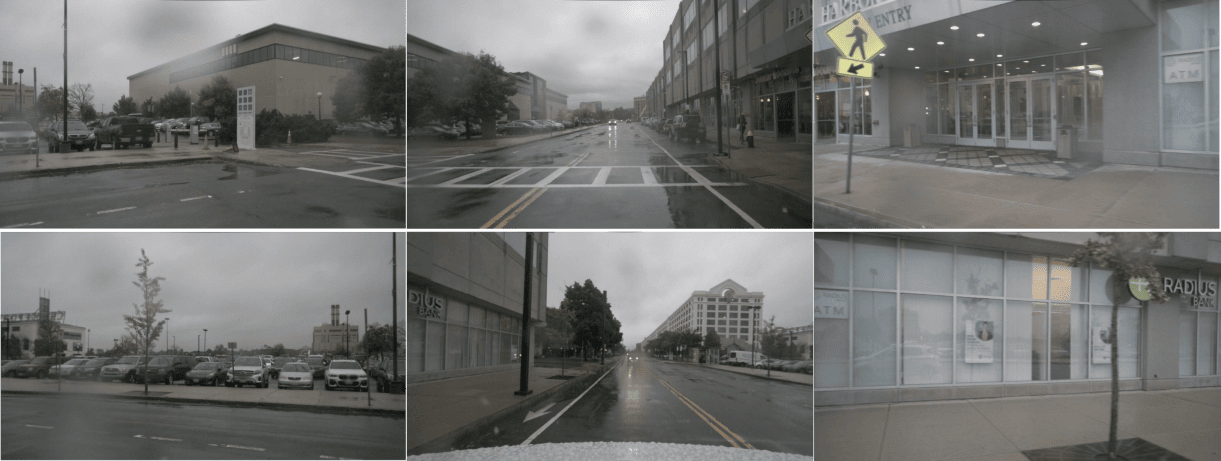
\includegraphics[width=0.9\linewidth]{src/description_exp1.png}
\end{center}

\vspace{1ex}

\noindent\textbf{\textcolor{purple}{Scene Style:}}
\begin{itemize}[leftmargin=15pt, itemsep=2pt]
    \item \textcolor{blue}{Time of the day}: daytime, with diffused lighting due to cloud cover
    \item \textcolor{blue}{Weather}: light to moderate rain, as indicated by raindrops on the camera lens and wet pavement
    \item \textcolor{blue}{Surrounding environment}: urban street flanked by mixed-use buildings and parking areas
    \item \textcolor{blue}{Road condition}: long, straight, two-lane road with clearly marked crosswalks and lane dividers; visibly slick from rainfall


\end{itemize}

\noindent\textbf{\textcolor{purple}{Foreground Objects:}}
\begin{itemize}[leftmargin=15pt, itemsep=2pt]
  \item \textcolor{blue}{Cars (left side)}: a variety of parked vehicles, including a dark pickup truck, compact sedans, SUVs, and so on, aligned parallel along the sidewalk; some cars have reflections on the wet ground
  \item \textcolor{blue}{Cars (right side)}: several vehicles parked curbside in front of commercial buildings, including economy cars to midsize SUVs
  \item \textcolor{blue}{Pedestrian}: an individual wearing a bright orange reflective safety vest and holding a red umbrella, standing near a crosswalk, suggesting a crossing action in progress
  \item \textcolor{blue}{Traffic cone}: bright orange cone placed on the sidewalk near the edge of a parking entrance, likely for safety or to reserve space
  \item \textcolor{blue}{Traffic sign}: a yellow pedestrian crossing sign mounted on a pole; the sign is positioned close to a glass-door building entrance
\end{itemize}

\noindent\textbf{\textcolor{purple}{Background Elements:}}
\begin{itemize}[leftmargin=15pt, itemsep=2pt]
  \item \textcolor{blue}{Road}: appears dark and glossy due to recent rainfall; lane markings and crosswalks are clearly visible
  \item \textcolor{blue}{Sidewalk}: wide, concrete sidewalks run alongside the road, bordered by planters and lined with trees
  \item \textcolor{blue}{Buildings}: prominent structures include multi-level modern commercial buildings with large glass façades
  \item \textcolor{blue}{Trees}: scattered urban landscaping includes small trees planted at regular intervals, offering a touch of greenery
  \item \textcolor{blue}{Car Parking}: multiple designated parking areas, some directly along the street and others within enclosed lots
  \item \textcolor{blue}{Crosswalk}: wide white-striped pedestrian crossings present at intersections
  \item \textcolor{blue}{Streetlights}: installed at intervals along the road to provide visibility during low-light conditions
\end{itemize}

\noindent\textbf{\textcolor{purple}{Scene-Graph Layout:}}
\begin{center}
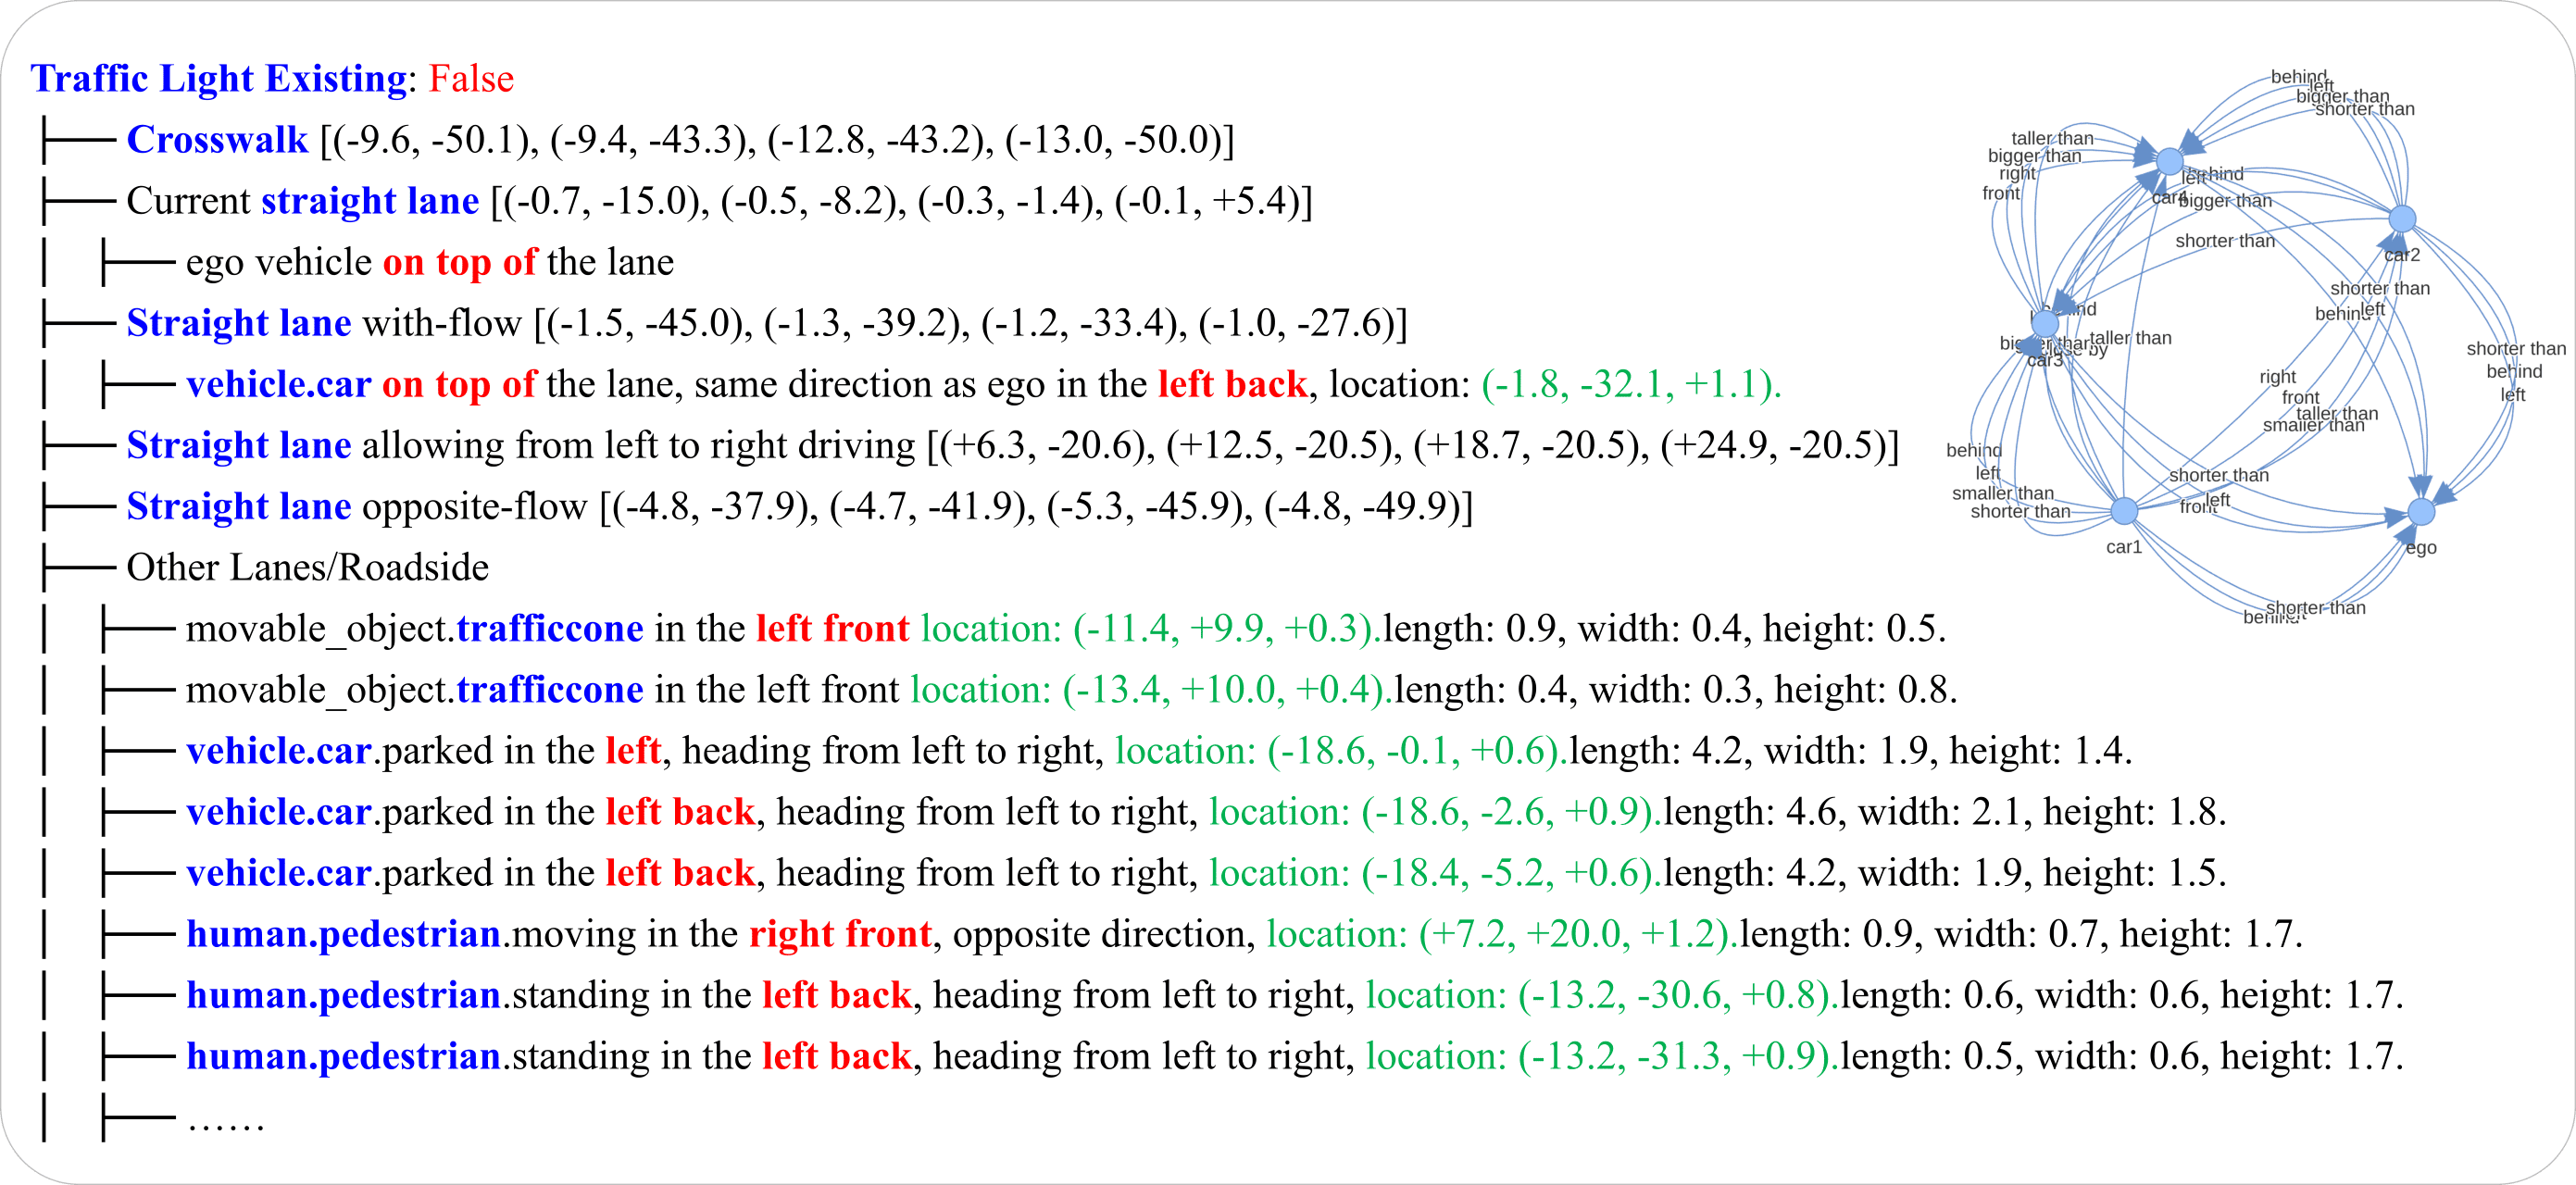
\includegraphics[width=0.98\linewidth]{src/layout1.png}
\end{center}


\noindent\textbf{\textcolor{purple}{Abstract Description:}}
\begin{itemize}[leftmargin=15pt, itemsep=2pt]
  \item \textcolor{gray!10!black}{The scene shows a rainy day on an urban expressway with wet roads reflecting light. Numerous cars are parked on both sides of the street, and a pedestrian in a bright orange safety vest is near the crosswalk. The background features multi-story commercial buildings with large windows, trees lining the sidewalk, and various signage. Streetlights are visible, and the area is marked with crosswalks and lane lines, creating a realistic and structured urban driving scene.}
\end{itemize}

\end{tcolorbox}
